\cotefile{154}
\scanpage{62}
% archive sheet number: 61
% printed form
{\ttfamily\small\raggedright
\$HASP373 STARTED - INIT 2 - CLASS 1 - SYS E333\\
IEF236I ALLOC. FOR CRAY2\\
IEF142I CRAY2 - STEP WAS EXECUTED - COND CODE 0000\\
IEF373I STEP / \hspace{1em} / START 82229.0906\\
IEF374I STEP / \hspace{1em} / STOP 82229.0906 CPU 0MIN 00.01SEC SRB 0MIN 00.00SEC VIRT 8K SYS 200K\\
IEF375I JOB /CRAY2 \hspace{1em} / START 82229.0906\\
IEF376I JOB /CRAY2 \hspace{1em} / STOP 82229.0906 CPU 0MIN 00.01SEC SRB 0MIN 00.00SEC\par}

\diagram{\handwritten{\begin{tikzcd}[ampersand replacement=\&,column sep=large]
 F=F_D \arrow[r] \& F_{D'}=F'
\end{tikzcd}}}

\figure{\handwritten{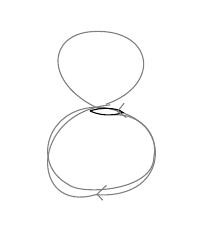
\begin{tikzpicture}[scale=.7]
\draw[thin,gray] (0,.04) .. controls (-1,.5) and (-.94,1.4) .. (-.1,1.44)
 .. controls (.98,1.5) and (1.16,.48) .. (.13,.12);
\draw[gray] (.1,.06) .. controls (-.9,.16) and (-1.27,-.94) .. (-.56,-1.33)
 .. controls (-.35,-1.53) and (.99,-1.47) .. (1,-.84)
 .. controls (1.1,-.32) and (.63,-.04) .. (.1,.06);
\draw[thin,gray] (.21,.11) .. controls (-1.28,-.03) and (-1.24,-1.87) .. (-.06,-1.52)
 .. controls (1.4,-1.62) and (1.26,-.03) .. (.28,-.07);
\draw (-.16,0) .. controls (.04,.07) and (.34,.06) .. (.44,-.03)
 .. controls (.24,-.1) and (0,-.08) .. (-.16,0);
\draw[thin,gray] (.46,.14)--(.34,-.01)--(.5,-.12);
\draw[thin,gray] (.14,-1.35)--(-.03,-1.51)--(.07,-1.62);
\end{tikzpicture}}}

\diagram{\handwritten{\begin{tikzcd}[ampersand replacement=\&,column sep=7em,row sep=2.4em]
\omega(F_D) \arrow[r,"{\alpha\ \text{transport parallèle}}","{\text{cond. via les}\ \mathrm{Pol}(D)}"'] \arrow[d,phantom,"\rotatebox{90}{$\simeq$}" description] \& \omega(F_{D'}) \arrow[d,phantom,"\rotatebox{90}{$\simeq$}" description]\\
\omega(\deleted{\unsure{\partial}}F\deleted{\unsure{,}}) \arrow[r,"{\beta\ \text{transport de}}","{\text{l'orientation sur }\unsure{\mathscr X|X|\mathcal X}}"'] \arrow[d,phantom,"\rotatebox{90}{$\simeq$}" description] \& \omega(F') \arrow[d,phantom,"\rotatebox{90}{$\simeq$}" description]\\
\omega(D) \arrow[r,"{\alpha'\ \text{transport parallèle}}"] \& \omega(D')
\end{tikzcd}}}

\figure{\handwritten{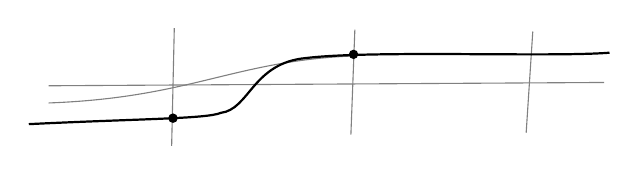
\begin{tikzpicture}[x=.84cm,y=.84cm]
\draw[thin,gray] (0,.48)--(8.4,.53);
\draw[thin,gray] (0,.22) .. controls (2.15,.3) and (2.78,.85) .. (4.58,.93);
\draw[thin,gray] (1.86,-.43)--(1.90,1.35) (4.57,-.26)--(4.63,1.33) (7.22,-.23)--(7.32,1.3);
\draw[thick] (-.3,-.1) .. controls (1.34,-.02) and (2.4,-.02) .. (2.6,.07)
 .. controls (3.04,.12) and (3.08,.83) .. (3.9,.9)
 .. controls (4.9,1.02) and (7.6,.91) .. (8.48,.98);
\fill (1.88,-.01) circle (.072) (4.61,.955) circle (.071);
\end{tikzpicture}}}

\handwritten{$\alpha=\alpha'$, \quad $\beta=\alpha,\alpha'$ ssi nb d'opérations \inserted{$N$} est pair}

\handwritten{\uline{ex} \quad $F=F_{D'}$, \quad $\alpha=\alpha'=-1$ \quad alors $\beta=-1$ ssi \deleted{\unsure{nb|tel}} $N$ pair}

\handwritten{donc}
\scanpage{63}
% archive sheet number: 62
et tout chemin \inserted{$c$} définit des iso. d'ens à deux éléments
\diagram{\begin{tikzcd}[ampersand replacement=\&,column sep=large,row sep=small]
\underline{\omega}(\deleted{\unsure{D}}F)\simeq\underline{\omega}(D) \arrow[r,"{\underline{\omega}_X(c)}"] \& \underline{\omega}(\deleted{\unsure{D}}F')\simeq\underline{\omega}(D')\\
\unsure{\varepsilon_s|\underline{\varepsilon}_s}(F)=\varepsilon_s(D) \arrow[r] \& \varepsilon_s(F')\simeq\varepsilon_s(D')\\
\varepsilon_{a}(F)\simeq\varepsilon_a(D)\arrow[r] \& \varepsilon_a(F')\simeq\varepsilon_a(D')
\end{tikzcd}}

Ces ens. ne sont pas indépendants, chaque paire de deux détermine le troisième, par la relation
\[
\underline{\omega}(F)\simeq\varepsilon_s(F)\wedge\varepsilon_a(F)
\]
et les deux relations similaires équivalentes. Au niveau des caractères correspondants sur $\pi_1(\mathscr{X},F)$, cela donne
\[
\begin{aligned}
&\boxed{\chi_X(F)=\chi_s(F)\chi_a(F)}\\
&\overset{\shortparallel}{\underset{\underline{\omega}(D)}{\underset{\shortparallel}{\chi_X(D)}}}=\chi_s(\overset{\shortparallel}{D})\chi_a(D)
\end{aligned}
\]
ou de façon plus symétrique
\[
\chi_X(F)\rho_s(F)\chi_a(F)=1
\]

En plus de ces trois caractères, il y en a deux autres, $\chi_{\mathscr X}$ = caractère d'\unsure{orientabilité|orientation} de $\mathscr X$ (ne dépendant pas de la structure cellulaire), et $\chi_c$ (``combinatoire''), qui est donné par la parité \inserted{des côtés}\inserted{Attention, dans le \unsure{compte des points|points|parité}, \deleted{\unsure{du poids|est fixé}} il faut compter pour \uline{deux} le franchissement de \unsure{tout|d'un|d'une} côté except.$^{\mathrm{el}}$ (qui \unsure{au schéma|au schème|amorce un demi-tour}, se décompose en effet en deux opérations)}.
% slanted
\deleted{Le système local associé est les} \inserted{Le correspondant est défini par les} $\underline{\omega}(F)$, mais en $y$ affectant les transitions \uline{opposées} à celles données par \deleted{\unsure{identifications}} le transport parallèle sur $X$ défini par les $\underline{\omega}_X(c)$ -- donc on aura
\[
\underline{\omega}_{\mathscr X}(c)=\mathrm{par}(c)\,\omega_X(c)
\]
où $\mathrm{par}(c)$ désigne la parité de $c$.

\deleted{\unsure{En résumé|Le système}} Le système local associé à $\chi_c$ est \deleted{formé de} comme fibres les ens standards $\{\pm1\}$, mais les morphismes de transition donnés par les $\mathrm{par}(c)$. On a donc
\[
\boxed{\chi_{\mathscr X}=\chi_o\chi_c}.
\]
% slanted
\margin{On a $\chi_c=1$ cf page suivante !}

En résumé, compte tenu de ces relations, on dispose de trois caractères fondamentaux \inserted{parmi les cinq}, je choisis
\[
\chi_X,\chi_s,\chi_c
\]
donc les deux autres sont
\[
\chi_a=\chi_X\chi_s\quad\text{et surtout}\quad\chi_{\mathscr X}=\chi_X\chi_c.
\]

Il y a lieu d'expliciter les valeurs des caractères \unsure{principaux|précéd.|précédents}, si faire se peut, ainsi que celles des la Représentation
\[
u:\pi_1(\mathscr X,F_D)\longrightarrow\operatorname{Aut}(\mathrm{Pol}(D)),
\]
\scanpage{64}
% archive sheet number: 63
% @ L1–2
sur les circuits fondamentaux sur $\mathscr X$, qui sont de deux espèces

% @ L3–7, a)
a) \inserted{demi} circuit autour d'une \deleted{\unsure{droite|arête}}\inserted{composante} exceptionnelle de $K$ (en la traversant \deleted{une} \unsure{fois|fois ?}), soit $l_{\underline D_i}$ le circuit correspondant : la \unsure{psdroite|ps.\ droite} $D_i\in\Sigma$. On trouve
\[
u(l_{\vec D_i})=\text{translation par }n-1
\]
% @ L8–11
(dans le sens de l'orientation de la position rel.$^{\unsure{t|\acute e}}$ \unsure{à} $D$ voisine de $D_i$), valeurs des caractères fondamentaux
\[
\chi_X(l_{\underline D_i})=+1,\quad\chi_s(l_{\underline D_i})\underset{*}{=}\deleted{\unsure{+}}(-1)^{n-1},\quad\deleted{\chi_c(l_{\underline D_i})=1}
\]
% @ L12–17, b)
b) Demi-circuit autour d'un pt \deleted{de} $X$ (qui peut être soit dans une face, soit dans un côté, soit \inserted{être} un sommet). La \deleted{point} \unsure{feuillet|feuillets|facette|effet} de ce point dans $\mathrm{Pol}(D)$ reste \unsure{fixe|figée} pour $u(l)$, qui est de signe $-1$, donc on trouve toutes les symétries, donc
\[
u_D:\pi_1(\mathscr X,F_D)\longrightarrow\operatorname{Aut}(F_D)
\]
% @ L19
est \uline{surjectif} \quad ouf !

% @ R1–9, asterisk
$*$ Il semble que le caractère $\chi_c$ soit \uline{trivial} ! En effet, si pour une p.v. $D$ donnée, on désigne par $\mathrm{sing}_D$ (``singularité de $D$'') le nb de sommets de $\Sigma$ qu'elle contient, je dis que pour un chemin $c$ qui va de $D$ en $D'$, on a
\[
\mathrm{poids}\ c\equiv\mathrm{sing}_{D'}-\mathrm{sing}_D\qquad(2)
\]
% @ R10–15
(donc poids $c$ \uline{pair} si $D=D'$!) On est ramené au cas où $c$ est de longueur $1$, auquel cas cette formule est triviale. (en se rappelant que pour le franchissement \deleted{d'une d.} en ``balayage'' au dessus d'une \deleted{droite} $D_i\in\Sigma$, le poids est 2.

% @ R16–19
Donc finalement, \uline{on trouve}
\[
\boxed{\chi_{\mathscr X}=\chi_X\ -}
\]
il n'y a pas d'autre caractère à regarder que ceux provenant de $\mathbb D_2$ !
\scanpage{65}
% archive sheet number: 64
% @ upper left, date
3.1.84

% @ upper left, first surface
\figure{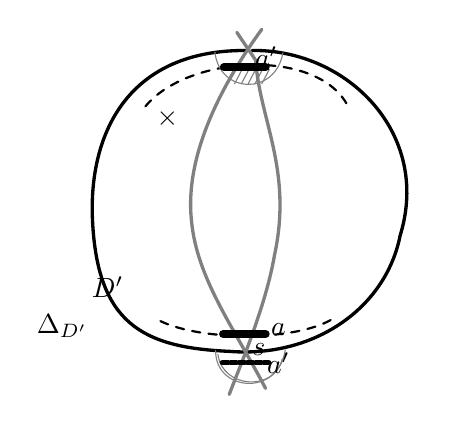
\begin{tikzpicture}[x=.96cm,y=.96cm,line cap=round,line join=round]
\draw[very thick] (0,2) .. controls (-1.52,2.01) and (-2.08,.95) .. (-2.03,-.23) .. controls (-1.97,-1.6) and (-1.38,-1.93) .. (-.22,-1.98) .. controls (.9,-2.07) and (1.85,-1.41) .. (2.04,-.45) .. controls (2.46,.91) and (1.33,2.02) .. (.08,2);
\draw[very thick,gray] (.21,2.28) .. controls (-.24,1.66) and (-.82,.68) .. (-.72,-.25) .. controls (-.65,-1.02) and (-.15,-1.68) .. (.26,-2.47);
\draw[very thick,gray] (-.12,2.24)--(.13,1.87) .. controls (.18,1.09) and (.62,.42) .. (.38,-.7) .. controls (.26,-1.4) and (-.09,-2.2) .. (-.22,-2.55);
\draw[thick,dashed] (-1.33,1.26) .. controls (-.78,1.93) and (.9,2.04) .. (1.33,1.3);
\draw[thick,dashed] (-1.13,-1.58) .. controls (-.57,-1.85) and (.71,-1.85) .. (1.18,-1.53);
\draw[gray] (-.41,1.98) .. controls (-.35,1.42) and (.39,1.4) .. (.49,1.97);
\draw[gray] (-.4,-1.97) .. controls (-.41,-2.51) and (.43,-2.59) .. (.52,-1.96);
\draw[gray] (-.37,-2.02) .. controls (-.31,-2.48) and (.39,-2.51) .. (.48,-2.08);
\foreach \x in {-.24,-.15,-.06,.03,.12,.21}{\draw[thin,gray] (\x,1.56)--++(.10,.19);}
\draw[line width=3pt] (-.29,1.78)--(.26,1.78) (-.30,-1.75)--(.26,-1.75);
\draw[line width=2pt,densely dotted] (-.31,-2.13)--(.30,-2.13);
\node at (-1.04,1.10) {$\times$};\node at (.27,1.91) {$a'$};
\node at (.43,-1.69) {$a$};\node at (.43,-2.13) {$a'$};\node at (.17,-1.95) {$s$};
\node at (-1.83,-1.13) {$D'$};\node at (-2.43,-1.65) {$\Delta_{D'}$};
\end{tikzpicture}\hspace{.55em}
% @ upper centre, second surface
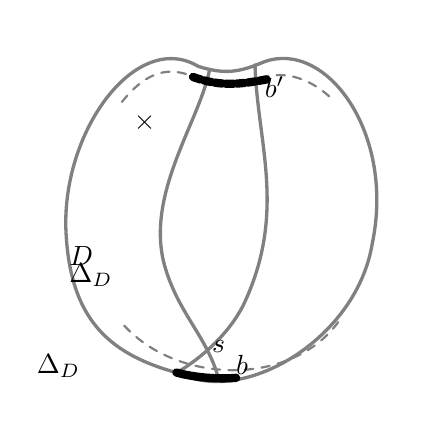
\begin{tikzpicture}[x=.96cm,y=.96cm,line cap=round,line join=round]
\draw[very thick,gray] (-.36,2.04) .. controls (-1.18,2.53) and (-2.18,1.18) .. (-2.11,-.16) .. controls (-2.05,-1.35) and (-1.5,-1.79) .. (-.58,-2.03) .. controls (.25,-2.43) and (1.73,-1.57) .. (1.94,-.31) .. controls (2.25,1.16) and (1.33,2.4) .. (.51,2.10) .. controls (.18,1.96) and (-.01,1.93) .. (-.36,2.04);
\draw[very thick,gray] (-.21,2) .. controls (-.34,1.32) and (-1.06,.36) .. (-.81,-.58) .. controls (-.64,-1.2) and (-.27,-1.51) .. (-.11,-2.03);
\draw[very thick,gray] (.39,2.06) .. controls (.42,1.02) and (.82,.1) .. (.23,-1.13) .. controls (-.01,-1.59) and (-.44,-1.89) .. (-.64,-2.01);
\draw[thick,dashed,gray] (-1.37,1.57) .. controls (-.91,2.15) and (-.57,1.94) .. (-.38,1.9);
\draw[thick,dashed,gray] (.46,1.89) .. controls (.82,1.99) and (1.14,1.87) .. (1.43,1.59);
\draw[thick,dashed,gray] (-1.34,-1.39) .. controls (-.61,-2.18) and (.89,-2.19) .. (1.50,-1.33);
\draw[line width=3pt,densely dotted] (-.43,1.9) .. controls (-.05,1.76) and (.23,1.81) .. (.56,1.87);
\draw[line width=3pt] (-.65,-2.01) .. controls (-.4,-2.08) and (-.08,-2.1) .. (.14,-2.08);
\node at (-1.07,1.29) {$\times$};\node at (.65,1.77) {$b'$};\node at (.22,-1.91) {$b$};\node at (-.09,-1.66) {$s$};
\node at (-1.91,-.47) {$D$};\node at (-1.78,-.72) {$\deleted{\unsure{\Delta_D}}$};\node at (-2.21,-1.92) {$\Delta_D$};
\end{tikzpicture}}

% @ L1–6 under drawings
huit façons ``standard'' de vriller $\Delta_D$ à $\Delta_{D'}$ suiv.$^{\mathrm t}$ \deleted{la} \deleted{une} isom. \unsure{(orienté)|(orient.)|(combinatoire)} d'un des deux arcs de transition \inserted{$a,a'$} sur $\Delta_{D'}$, avec l'un des deux arcs privilégiés $b$ (de transition) et $b'$ (son antipodique) sur $\Delta_D$, deux choix pour chaque choix d'un couple dans $\{a,a'\}\times\{b,b'\}$.

% @ L6–12 to R7
Donc huit façons à priori de construire une surface \inserted{cellulaire} ayant pour graphe $\Gamma_{\underline\Sigma}=\Gamma$, mais (sauf pour les \unsure{plongements|polygones} d'\unsure{un complexe|une courbe|un couloir} rouge, \unsure{différent|différents}) il n'y a que quatre cas différents de surfaces, car ce qu'on obtient par un choix $(\alpha,\beta,\unsure{\varphi|\sigma|\rho})$\inserted{iso. de recollt} et $(\alpha',\beta',\sigma')$ (où $\alpha',\beta',\sigma'$ déduits en composant avec les antipodismes) sont can. isom. (ils correspondent à la \ensuremath{=} circularisation de $\Gamma$, et les $\mathord{=}$ \unsure{réflexions|morphismes|multiplicateurs} de transition pour les or. loc. correspond. de ).

% @ R8–20
On peut en supposer, quitte à composer avec les antipodismes de part et d'autre, que $\beta=b$ -- ce qui revient à faire un choix où le sommet $s$ apparaît \deleted{\unsure{sur}} au voisinage de l'arc de transition choisi, sur la surface \unsure{vrillée|recollée} (au lieu qu'il soit rejeté aux antipodes, ce qui a l'air un peu idiot !)

% @ R, last two lines
\deleted{Pour les quatre choix (en fait, les huit)} qui
\scanpage{66}
% archive sheet number: 65
% @ L1–5, cancelled continuation
\deleted{\deleted{\unsure{sont}} envisageables il y a une application canonique de la surface vrillée dans $X$ ! \deleted{Si on recolle par} \inserted{Non, c'est vrai pourvu} \deleted{\unsure{donc|dès}} que, pour $\alpha$ choisi, on choisisse l'identification}

% @ L6–12
Si on veut une application naturelle de la surface vrillée dans $X$, qui sur $\Delta_D,\Delta_{D'}$ se réduise au plongement canonique, il faut \inserted{(semble-t-il)} que $b$ et $\alpha$ se réalisent par le $=$ segment plongé dans $X$, ce qui \inserted{semble} imposer $\alpha=a'$ ! Mais si on convient de remplacer $\Delta_D$ par un disque un peu plus petit $\Delta_D^*$ \inserted{dont le bord} passant par $s$ (cf pointillé ci-contre), et déplace en conséquence $b$ en $b^*$, et faire le vrillement le long de $b^*$ plutôt que $b$, \deleted{donc} et pareil pour le disque $\Delta_{D'}$,

% @ L, inset beside passant par s
\figure{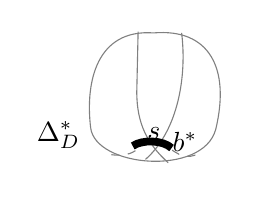
\begin{tikzpicture}[x=.85cm,y=.85cm]
\draw[gray] (0,.98) .. controls (-.85,1.04) and (-1.02,.25) .. (-.94,-.43) .. controls (-.88,-1.03) and (.74,-1.17) .. (.93,-.46) .. controls (1.15,.46) and (.83,1.05) .. (0,.98);
\draw[gray] (-.23,1)--(-.25,.1) .. controls (-.25,-.38) and (-.09,-.68) .. (.22,-.96);
\draw[gray] (.42,.98) .. controls (.5,.34) and (.37,-.48) .. (-.12,-.91);
\draw[thin,dashed,gray] (-.63,-.84) .. controls (-.23,-.89) and (-.22,-.66) .. (0,-.64) .. controls (.24,-.65) and (.36,-.97) .. (.66,-.83);
\draw[line width=2.8pt] (-.31,-.71) .. controls (-.17,-.61) and (.14,-.62) .. (.27,-.74);
\node at (.005,-.52) {$s$};\node at (.47,-.65) {$b^*$};\node at (-1.42,-.55) {$\Delta_D^*$};
\end{tikzpicture}}

% @ L, final five lines
(de façon à faire \unsure{coïncider|coincider} les images de $a$ et $a'$ dans $X$), on voit qu'on arrivera à \deleted{faire appliquer} \inserted{trouver} une application de la surface vrillée dans $X$, même en choisissant $\alpha=a$.

% @ L last line to R1–3
Le choix le plus naturel quand même (\deleted{dans} pt de vue application dans $X$) semblerait $\alpha=a'$. Donc sur le terrain cela donne -- \uline{continuation}

% @ R, below continuation
\figure{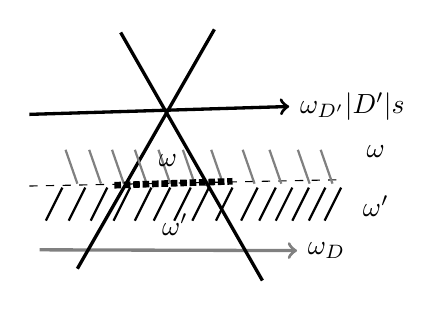
\begin{tikzpicture}[x=1cm,y=1cm]
\draw[->,very thick] (-1.75,.76)--(1.55,.86) node[right] {$\unsure{\omega_{D'}|D'|s}$};
\draw[->,very thick,gray] (-1.62,-.96)--(1.65,-.97) node[right,black] {$\omega_D$};
\draw[very thick] (-1.14,-1.2)--(.60,1.84) (-.59,1.8)--(1.21,-1.35);
\draw[dashed,thin] (-1.75,-.15)--(2.2,-.07);
\foreach \x in {-1.14,-.84,-.55,-.26,.04,.35,.71,1.11,1.45,1.81,2.1}{\draw[thick,gray] (\x,-.12)--++(-.15,.43);}
\foreach \x in {-1.33,-1.04,-.76,-.47,-.2,.04,.3,.53,.83,1.15,1.38,1.59,1.8,2.01,2.21}{\draw[thick] (\x,-.17)--++(-.21,-.42);}
\draw[line width=2.4pt,densely dotted] (-.67,-.14)--(.83,-.09);
\node at (.01,.18) {$\omega$};\node at (.10,-.64) {$\omega'$};
\node at (2.65,.29) {$\circlearrowleft\omega$};\node at (2.65,-.4) {$\circlearrowleft\omega'$};
\end{tikzpicture}}
% @ R4–8
d'une rive par la suivante -- l'application $\mathscr X\to X$ est une \uline{immersion}.

% @ R9–end
Dans cette optique \inserted{donc}, la rive de $D'$ i.e. l'arc sur $\partial\Delta_{D'}$ qui exprime l'opération de \deleted{spécialisation}\inserted{générisation} vers $D$ est $a'$ -- i.e. celle qui ``fait face'' à la rive $a$, et non à qui en est déduite par ``transport parallèle'' au cours de la déformation de spécialisation $D\longrightarrow D'$. Ce choix semble parfaitement naturel -- l'ennui,
\scanpage{67}
% archive sheet number: 66
% @ L1–5
c'est qu'il semble que sur la carte $\mathscr X$ obtenue par vrillement, on n'ait aucune interprétation des ``trous'' (ou sommets, quand on a bouché les trous) en termes de la géométrie de $\underline{\Sigma}$.

% @ L6–10
\deleted{\unsure{C}} Il faudrait quand même que je réessaye, pour voir si je \deleted{\unsure{né|ne}} m'étais pas mélangé les pinceaux $\ldots$ \deleted{\unsure{I}} Quand on a fait ce vrillement, et qu'on suit par continuité une orientation choisie

% @ L11–end
$\omega$ de $\Delta_D$ (définie par une or. $\omega_D$ de $D$) en passant de $\Delta_D$ dans $\Delta_{D'}$ via l'arc de transition, on trouve \deleted{que} une orientation $\omega'$ de $\Delta_D$, qui induit sur $D'$ une orientation, $\omega_{D'}$, qui est \uuline{opposée} de celle déduite par transport \deleted{\unsure{de structures}} parallèle ! Voilà donc rectifiée une erreur monumentale, commise dès les débuts !

% @ R1–7
Venons-en à l'autre choix qui donne lieu à $\mathscr X\to X$, savoir $\alpha=a$. On est obligé ici d'ajuster comme j'avais dit $\Delta_D,b$ et $(\Delta_{D'},a)$, pour faire se rencontrer $b$ et $a$ en $b^*\sim a^*\subset X$. On trouve la figure

% @ R, centre
\figure{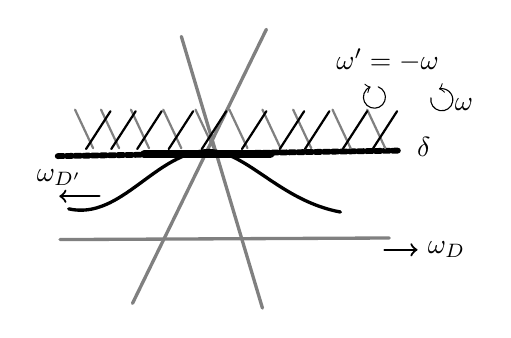
\begin{tikzpicture}[x=1cm,y=1cm,line cap=round]
\draw[very thick,gray] (-.40,1.55)--(.63,-1.9) (.68,1.64)--(-1.02,-1.84);
\draw[very thick,gray] (-1.94,-1.03)--(2.24,-1.01);
\draw[thick,->] (2.18,-1.16)--(2.60,-1.16) node[right] {$\omega_D$};
\draw[very thick] (-1.83,-.64) .. controls (-1.16,-.79) and (-.72,.10) .. (-.04,.10) .. controls (.44,.08) and (.86,-.54) .. (1.62,-.68);
\draw[thick,->] (-1.44,-.48)--(-1.95,-.48) node[above] {$\omega_{D'}$};
\draw[line width=2.1pt,densely dotted] (-1.97,.03)--(2.35,.10);
\draw[line width=3pt] (-.87,.055)--(.73,.055);
\foreach \x in {-1.52,-1.19,-.81,-.4,.01,.44,.86,1.25,1.75,2.19}{\draw[thick,gray] (\x,.13)--++(-.23,.49);}
\foreach \x in {-1.61,-1.29,-.96,-.56,-.14,.37,.85,1.17,1.65,2.03}{\draw[thick] (\x,.12)--++(.31,.48);}
\node at (2.68,.15) {$\delta$};
\draw[->] (2.1,.91) arc (70:-250:.14);
\node at (2.22,1.25) {$\omega'=-\omega$};
\draw[->] (2.77,.77) arc (170:465:.14);
\node at (3.19,.69) {$\omega$};
\end{tikzpicture}}

% @ R, below figure
i.e. on \unsure{vrille|recolle} avec elle-\ensuremath{=} \uline{la $=$ rive} \deleted{de} le long de la ligne critique de spécialisation $\delta$. L'identification $b^*\to a^*$, comme tantôt, est l'iso de transport. Ici, la combinatoire (choix \inserted{d'orien$\unsure{\mathrm t|\mathrm n}$} de structure polygonale sur l'arc de transition associé à une p.v.) est sujette au choix opposé
\scanpage{68}
% archive sheet number: 67
% @ L1–9
de tantôt, pour \unsure{répérer|repérer} une op. de générisation $D'\longrightarrow D$ par un ``arc de \deleted{\unsure{spécial|spécialisation}}générisation'' sur $\partial\Delta_{D'}$ ; on prend maintenant, non la rive qui ``fait face'' à celle de $b$, mais par contre celle qui en résulte par transport parallèle. \deleted{Je \unsure{pensais}} \inserted{Quant à} l'isom. de transition $\underline{\omega}_{\Delta_D}\longrightarrow\underline{\omega}_{\Delta_{D'}}$ pour les orientations, faisant comme d'hab

% @ L10–11
\diagram{\begin{tikzcd}[ampersand replacement=\&,column sep=2em]
\omega\ \text{or. de }\Delta_D \arrow[r,leftrightarrow]\arrow[dr,to path={|- (\tikztotarget)\tikztonodes},"{\text{transport}}" near start,swap] \& \omega_D\ \text{or. de }D \& {}\\
{} \& \omega'\ \text{or. de }\Delta_{D'}\arrow[r,leftrightarrow] \& \omega_{D'}\ \text{or. de }D',
\end{tikzcd}}
% @ L12–14
on trouve à nouveau que $\omega_{D'}$ est \uline{opposée} à l'orientation \deleted{de $D$} déduite de $\omega_{D'}$ par transport parallèle !

% @ L15–end and R1–5
Pendant ces deux dernières semaines, c'est avec cette opération de vrillage que j'ai travaillé. Avant, j'avais pris \deleted{une} \uline{comme} iso. de transition pour les orientations le transport parallèle -- \deleted{\unsure{de façon}} et comme \deleted{\unsure{arcs}} vrillage, si je me rappelle bien, le vrillage $1^\circ)$ de $b$ avec $a'$ -- je croyais avoir interprété combinatoirement la construction de vrillement de $1^\circ)$, mais je m'étais mélangé les pinceaux de \uline{deux} façons, il me semble :

% @ R6–7
1) je m'étais trompé sur les isom. de transition pour les orientations, et

% @ R8–16
2) je m'étais trompé également sur l'identification correcte d'une op. de générisation \inserted{\unsure{pour|partt} $D'$} par un arc sur $\partial\Delta_{D'}$ -- en prenant au bonheur la chance celui qui \deleted{est} \deleted{\unsure{est}} se déduit de \uline{$b$} par transport parallèle, alors que c'est l'autre \deleted{qu'il} (l'antipodique, qu'il fallait prendre).

% @ R17–19
Pour résumer, les quatre possibilités sont indiqués dans la liste suivante
\scanpage{69}
% archive sheet number: 68
% @ L1–2
A) Recollements donnant lieu à une application naturelle
\[
\mathscr X\longrightarrow X,
\]
% @ L3–8
ou ce qui revient au $=$, où l'isom $\sigma:\alpha\longrightarrow\beta$ \inserted{(\deleted{\unsure{avec|moy.}} sans composer avec l'antipodisme)} est obtenu par transport parallèle -- ou aussi, combinatoirement, cas où l'isom de transition $\omega_D\longrightarrow\omega_{D'}$ est opposée au transport parallèle. Il y a deux possibilités (avec tjrs $\beta=b$)

% @ L9–13
1) Cas $\alpha=a'$ -- on \unsure{vrille|recolle} \deleted{l'arc de \unsure{sp}} \deleted{une rive $b$ de} l'arc de spéc $b$ sur $\Delta_D$ avec l'arc \deleted{$a'$ qui est} de gén. $a'$ sur $\Delta_{D'}$ qui est sur la rive \uline{faisant face} à celle de $b$, i.e opposée à celle obtenue par transport parallèle. \deleted{C'est} Alors $\mathscr X\to X$ est une immersion. \deleted{On repère}

% @ L14–19
\deleted{\unsure{C|On repère}} Pour définir la structure polygonale sur l'ens des transitions : à partir d'une p.v. donnée $D'$, on répère \deleted{\unsure{l'une des|d'une face}} \inserted{une op} de générisation par la rive qui est \deleted{\unsure{dans la direc|dans la direction}} celle vers laquelle on va déplacer $D'$ pour génériser : le trait bleu qui marque la rive ``tire'' sur $D'$ pour la déplacer vers lui.

% @ L20–21 to R6
2) Cas $\alpha=a$, -- on recolle $b$ avec l'arc $a$ qui s'en déduit par transport parallèle. Maintenant $\mathscr X\to X$ est une immersion sur chaque face $F^*$, mais c'est un rebroussement le long d'une frontière commune à deux faces.

% @ R7–17
On répère une op. de générisation par \deleted{la rive \unsure{li}} l'arc de gén. qui est opposé à la rive vers laquelle on se \unsure{pousse|dirige} -- le trait bleu marquant cette rive va venir ``pousser'' sur $D'$ pour la génériser, \deleted{et} la \unsure{détachant|détacher|direction} d'un sommet envisagé
\scanpage{70}
% archive sheet number: 69
% @ L1–7
B) Recollements \inserted{ne} donnant \uline{pas} lieu à une application naturelle $\mathscr X\to X$, i.e. l'isom $\sigma:\alpha\to\beta$ est \uline{opposé} à \unsure{celle|celui} obtenu par transp. par., ou par composition de celui-ci avec antipodisme -- ou encore, l'isom de transition $\underline{\omega}(D)\to\underline{\omega}(D')$ est \deleted{opposé à} celui du transport parallèle. Deux cas à envisager encore

% @ L8–14
1) Cas $\alpha=a'$. C'est le cas où on répère une op. de générisation \inserted{sur $D'$} par l'arc qui fait face à l'arc de spécialisation correspondant sur $D$ -- c'était un cas que pour une raison ou une autre j'avais écarté (c'était vraiment au bonheur-la-chance, rétrospectivement !).

% @ L15–end to R2
2) Cas $\alpha=a$ -- C'est le cas où on repère une op. de générisation par l'arc \inserted{de gén.} déduit de l'arc de spécialisation correspondant par transport parallèle. Je me suis amplement convaincu qu'il est impossible de ``suivre'' une p.v. en lui appliquant les itérés de l'opération \deleted{\unsure{\ensuremath{\rho}|\ensuremath{\beta}}} de ``tourner autour d'un trou (ou sommet \ldots).

% @ R3–14
Je crois me rappeler maintenant que j'avais écarté aussi le cas 1), car il donnait lieu aussi à des circuits qui avaient l'air idiots -- notamment en partant d'une p.v. proche d'une supersingulière, $D_i$, on s'écarte de $D_i$ au lieu de tourner autour comme on devrait normalement.

% @ R foot, cancelled lines; last line continues
\deleted{Là je viens de revérifier, cet ennui se présente aussi bien pour B 1) que pour B 2), et \unsure{ça|\ensuremath{=}} pour \deleted{\unsure{B}} A 1), et même, je viens de voir,} pour A 2 -- visiblement, dans ce dernier
\scanpage{71}
% archive sheet number: 70
% @ L1–9, crossed continuation at top
\deleted{cas au moins, c'est dû au fait que je n'ai pas tenu compte des arcs de spécialisations exceptionnels (vers leurs pos. supersingulières). Là encore, il y a deux variantes, \unsure{suivant|suivt} qu'on se permet de se spécialiser en une pos. rel supersingulière, ou qu'on veut l'éviter, en passant \deleted{directement} \unsure{à} la position voisine opposée}

% @ L10–18
Je viens de vérifier, sauf erreur (j'ai fait pas mal d'erreurs encore dans le cours de la vérification !) les trois procédés $A_1,A_2,B_{\unsure{1|3}}$ donnent lieu aux bons circuits \margin{\unsure{--\,.}}autour d'une position supersingulière, il n'y a que $B_2$ qui déconne complètement (or il semblerait que c'était sur $B_2$ que je m'étais arrêté pendant un jour ou deux, Dieu sait pourquoi !)

% @ L19–22
Le plus intéressant, après $A_2$, semble bien sûr $A_1$, mais je viens encore d'essayer de comprendre les circuits auxquels il donne naissance, sans y réussir.
\scanpage{72}
% archive sheet number: 71
% @ L1–9
Je voudrais revenir à la question de faire une surface avec les pos. \uline{stables}. Pour une telle $D$, $\Delta_D$ n'a comme arcs de transition que des arcs de \uline{spécialisation}. Comment raccorder $\Delta_D$ et $\Delta_{D'}$, quand $D,D'$ sont déduits l'un de l'autre par balayage au dessus d'un sommet ? Ici, il n'y

% @ L9–15, sketch between the two parts of the sentence
\figure{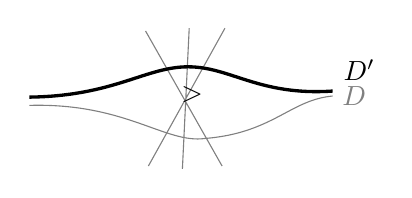
\begin{tikzpicture}[x=.72cm,y=.7cm]
\draw[gray] (-.6,-1.25)--(.75,1.25) (0,-1.3)--(.12,1.25) (.7,-1.25)--(-.65,1.2);
\draw[gray] (-2.7,-.15)..controls(-1,-.1)and(-.3,-.85)..(.4,-.75)..controls(1.6,-.65)and(1.9,-.05)..(2.65,.02) node[right]{$D$};
\draw[very thick] (-2.7,0)..controls(-1.2,.02)and(-.65,.55)..(.1,.55)..controls(.85,.55)and(1.35,.02)..(2.65,.11) node[above right]{$D'$};
\node at (.17,.05) {$>$};
\end{tikzpicture}}

% @ L9–20, text beside and below sketch
a pas d'ambiguïté possible sur les arcs le long desquels faire le vrillement, vu que l'interprétation de leur arc de spécialisation \unsure{n'en est plus une|n'est en plus une|et c'est plus utile} (il faudrait \unsure{du vis|du vice|du vif|être vicieux} pour l'utiliser pour vriller !). \margin{?} Ici, il est très tentant de remplacer encore $\Delta_D,\Delta_{D'}$ par $\Delta_D^*,\Delta_{D'}^*$ déduits en balayant le bord jusqu'au point $s$ ``critique'' qui nous intéresse, \deleted{avant} de vriller.

% @ L21–23 to R1–8
Résultat avec figures symétriques (à partir de la position \unsure{semi-stable|semi-stables|sous-stable} intermédiaire) on a à présent 8 possibilités

% @ R upper, two crossed drawings
\figure{\deleted{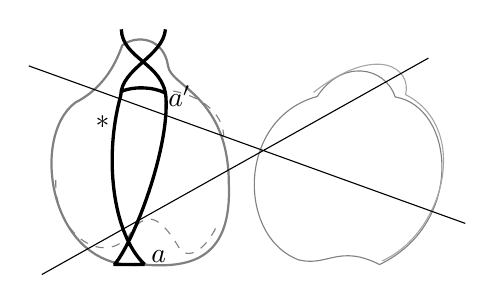
\begin{tikzpicture}[x=.66cm,y=.58cm]
\draw[gray,thick] (0,-2.2)..controls(-1.8,-2.4)and(-2.2,.6)..(-1.3,1.35)..controls(-.7,1.7)and(-.5,2.3)..(-.4,2.6)..controls(-.1,2.85)and(.4,2.75)..(.48,2.15)..controls(.52,1.7)and(1.65,1.5)..(1.65,-.45)..controls(1.7,-2)and(1,-2.3)..(0,-2.2);
\draw[gray,dashed] (-1.68,-.35)..controls(-1.72,-1.5)and(-.8,-2.25)..(-.28,-1.58)..controls(.05,-.95)and(.35,-1.15)..(.72,-1.89)..controls(1,-2.15)and(1.35,-1.6)..(1.45,-1.25) (.58,1.6)..controls(1.25,1.45)and(1.55,1)..(1.55,.6);
\draw[very thick] (-.42,2.95)..controls(-.4,2.3)and(.4,2.2)..(.44,1.45)..controls(.5,.35)and(-.15,-1.65)..(-.55,-2.2) (.43,2.95)..controls(.38,2.35)and(-.42,2.1)..(-.43,1.5)..controls(-.75,.2)and(-.61,-1.5)..(.03,-2.2) (-.42,1.59)..controls(-.2,1.7)and(.17,1.7)..(.42,1.56) (-.57,-2.2)--(.03,-2.2);
\node at (.7,1.48) {$a'$};\node at (.3,-2.02) {$a$};\node at (-.78,.92) {$*$};
\draw[gray] (3,-2.1)..controls(1.8,-1.6)and(1.8,1)..(3.35,1.48)..controls(3.82,2.3)and(4.65,2.15)..(4.85,1.47)..controls(6,1.25)and(6.2,-1.3)..(4.55,-2.2)..controls(3.77,-1.75)and(3.55,-2.25)..(3,-2.1);
\draw[gray!70] (3.28,1.57)..controls(4.5,2.65)and(5.18,2.1)..(5.05,1.52)..controls(6.3,.8)and(5.81,-1.5)..(4.6,-2.12);
\draw (-2.2,2.15)--(6.2,-1.3) (-1.95,-2.42)--(5.49,2.32);
\end{tikzpicture}}}

% @ R middle, redrawn pair of twists
\figure{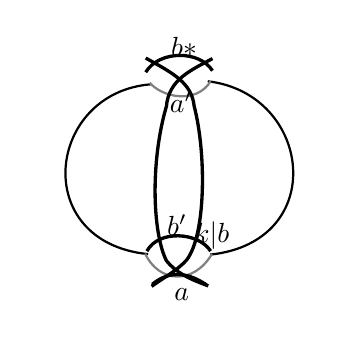
\begin{tikzpicture}[x=.75cm,y=.64cm]
\draw[thick] (-.48,1.53)..controls(-2.25,1.37)and(-2.55,-1.6)..(-.53,-1.84) (.48,1.59)..controls(2.25,1.35)and(2.55,-1.6)..(.52,-1.85);
\draw[gray,thick] (-.5,1.56)..controls(-.3,1.28)and(.28,1.12)..(.53,1.59) (-.58,-1.83)..controls(-.34,-2.42)and(.24,-2.45)..(.55,-1.84);
\draw[very thick] (-.57,2.05)..controls(-.12,1.76)and(.21,1.56)..(.25,1.1)..controls(.46,.15)and(.45,-1.47)..(.12,-1.96)..controls(-.04,-2.17)and(-.31,-2.34)..(-.47,-2.48) (.56,2.04)..controls(.18,1.8)and(-.18,1.62)..(-.22,1.09)..controls(-.49,.01)and(-.46,-1.4)..(-.22,-1.97)..controls(-.06,-2.2)and(.14,-2.32)..(.49,-2.47);
\draw[very thick] (-.57,1.77)..controls(-.34,2.21)and(.34,2.21)..(.56,1.8) (-.55,-1.78)..controls(-.35,-1.35)and(.32,-1.4)..(.53,-1.78) (-.46,-2.44)..controls(-.14,-2.13)and(.18,-2.23)..(.46,-2.45);
\node at (.08,2.28) {$b\deleted{*}$};\node at (.03,1.17) {$a'$};\node at (-.04,-1.26) {$b'$};\node at (.55,-1.47) {$\unsure{k|b}$};\node at (.04,-2.64) {$a$};
\end{tikzpicture}}

% @ R1–17 beside and below the redrawn figure
de vrillement, suivant les \deleted{qu'on} quatre choix d'\unsure{élémts|éléments} dans $\{a,a'\}\mathbin{\times}\{b,b'\}$, puis le choix d'orientation pour vriller $\alpha\in\{a,a'\}$ ou $\beta\in\{b,b'\}$. Mais déjà le choix d'un couple $(a,b')$ ou $(b,a')$ est exclu, à cause de la nécessaire symétrie à respecter. Donc il reste deux couples $(a,b)$, $(a',b')$, et pour chacun choix parmi les deux possibilités de vrillage -- transport parallèle, ou l'opposé. Mais modulo \deleted{application} transformation par antipodisme de part et d'autre (qui ne change pas la surface $X$ obtenue par vrillage \deleted{\unsure{suivant}} la disposition de la \deleted{\unsure{deux|droite|dedans}}) \unsure{DDS|reste|équivaut à} $(a,b)$.
\scanpage{73}
% archive sheet number: 72
% reading direction: sheet turned through 180 degrees
% printed form
% @ top of turned sheet, three printed lines
\noindent\texttt{/*JOB=CRAY2,ACCT=*********,ALL=M06,MSGL=N}\hfill\texttt{J0424CNU}\\
\texttt{// JOB MSGLEVEL=(1,1),MSGCLASS=A}\\
\texttt{// EXEC PGM=IEFBR14}

% @ top centre, beside form
\[\handwritten{N=4n}\]

% @ mathematical lines 1–3, across printed rules
\[
\begin{aligned}
&\handwritten{\sigma_0\;\sigma_1\; \text{---}\;\sigma_{N-1}\mid\sigma_N=\sigma_0}
&&\handwritten{\sigma_i^2=1}\\
&\handwritten{\rho_1=\sigma_0\sigma_1\quad\rho_2=\sigma_1\sigma_2\quad\text{---}\quad\rho_N=\sigma_{N-1}\sigma_N=\sigma_{N-1}\sigma_0}
&&\handwritten{\rho_i^2=1}\quad\text{\handwritten{si deux $\sigma_i$ consécutifs (circulairement) commut\unsure{ent|ent\deleted{s}}}}\\
&\handwritten{\rho_1\rho_2=\sigma_0\sigma_2\quad\rho_2\rho_3={}}
\end{aligned}
\]
% @ pencil sketches, turned page middle
\figure{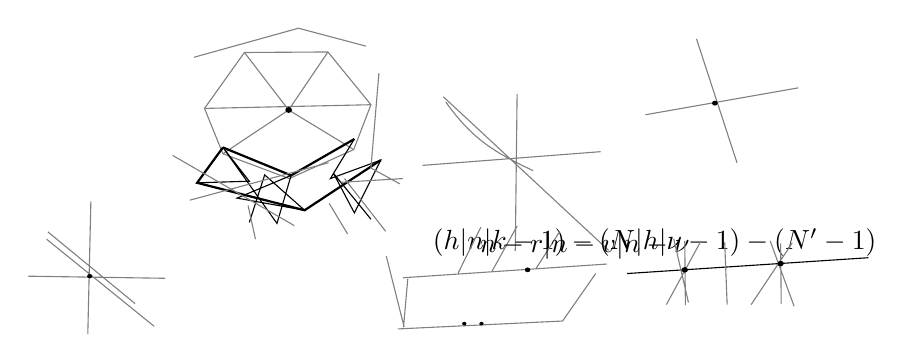
\begin{tikzpicture}[x=.78cm,y=.67cm]
\draw[gray] (1.3,2.55)--(3,3.1)--(4.1,2.76) (1.47,1.58)--(2.12,2.64)--(3.48,2.65)--(4.18,1.65)--(3.9,.8)--(2.85,.25)--(1.77,.72)--cycle;
\draw[gray] (2.12,2.64)--(2.84,1.55)--(3.48,2.65) (1.47,1.58)--(4.18,1.65) (1.77,.72)--(2.84,1.55)--(3.9,.8);
\fill (2.84,1.55) circle (.055);
\draw[thick] (1.77,.84)--(2.88,.31)--(3.91,1.0) (1.77,.84)--(1.35,.17)--(3.10,-.35)--(4.34,.6);
\draw (1.35,.17)--(2.20,.20)--(1.77,.84)--(2.65,-.6)--(2.88,.31)--(2.0,-.12)--(3.10,-.35)--(2.45,.32)--(2.2,-.58) (3.91,1.0)--(3.52,.25)--(4.34,.6)--(3.91,-.4)--(3.57,.35)--(4.18,-.52);
\draw[thin,gray] (.95,.69)--(2.93,-.64) (1.23,-.16)--(3.49,.55) (2.30,-.9)--(2.18,-.26) (3.8,-.8)--(3.5,-.22) (3.75,.25)--(4.42,-.75) (4.31,2.25)--(4.18,.45)--(4.65,.15) (3.7,.18)--(4.7,.25);
\draw[gray] (-1.1,-.9)--(.65,-2.55) (-.43,-2.7)--(-.38,-.18) (-1.4,-1.6)--(.83,-1.64) (-1.08,-.76)--(.34,-2.12);\fill(-.4,-1.6) circle(.042);
\draw[gray] (5.36,1.8)--(8.05,-1.11) (6.56,1.85)--(6.53,-1.12) (5.02,.5)--(7.92,.76) (5.4,1.7)..controls(5.84,.98)and(6.21,.74)..(6.82,.4);
\draw[gray] (8.65,1.46)--(11.14,1.97) (9.48,2.9)--(10.14,.55);\fill(9.78,1.68) circle(.047);
\node at (8.8,-.97) {\handwritten{$(\unsure{h|n|k}-1)-(\unsure{N|h|\nu}-1)-(N'-1)$}};
\draw[gray] (4.62,-2.6)--(7.3,-2.45)--(7.84,-1.55) (4.72,-2.56)--(4.43,-1.22) (4.71,-2.57)--(4.78,-1.65) (4.7,-1.63)--(8.02,-1.37) (5.6,-1.54)--(5.97,-.67) (6.15,-1.51)--(6.56,-.65) (6.86,-1.47)--(7.25,-.76);
\fill(6.73,-1.48) circle(.045);\fill(5.7,-2.5) circle(.035);\fill(5.98,-2.5) circle(.035);
\node at (7.66,-1.02) {\handwritten{$\unsure{n-r|n-v|n-\nu}$}};
\draw (8.35,-1.55)--(12.28,-1.25);\draw[gray] (9.11,-.89)--(9.35,-2.1) (8.99,-2.14)--(9.55,-.94) (9.30,-2.15)--(9.29,-.93) (9.94,-.96)--(9.98,-2.14) (10.37,-2.14)--(11.04,-.97) (10.68,-.93)--(11.07,-2.17) (10.86,-2.12)--(10.85,-.98);
\fill(9.29,-1.48) circle(.052);\fill(10.85,-1.36) circle(.052);
\end{tikzpicture}}
\scanpage{74}
% archive sheet number: 73
% @ top left, four directed horizontal strokes and crossing slants
\figure{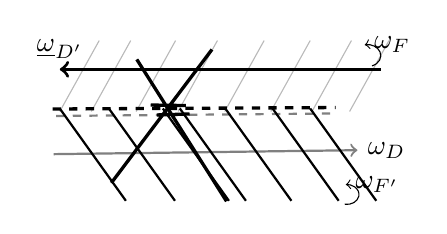
\begin{tikzpicture}[x=.77cm,y=.63cm]
\foreach \x in {0,.52,1.26,1.95,2.72,3.48,4.16,4.78}{\draw[gray!55] (\x,.6)--++(.65,1.43);}
\draw[very thick,<-] (0,1.45) node[above]{$\underline\omega_{D'}$}--(5.3,1.45);
\draw[very thick,dashed] (-.12,.65)--(4.55,.68);\draw[thick,dashed,gray] (-.06,.51)--(4.54,.56);
\draw[gray,thick,->] (-.1,-.26)--(4.91,-.18) node[right,black]{$\omega_D$};
\foreach \x in {0,.81,1.7,1.98,2.73,3.51,4.13}{\draw[thick] (\x,.66)--++(1.09,-1.86);}
\draw[very thick] (1.27,1.65)--(2.75,-1.21) (.85,-.84)--(2.51,1.85) (1.5,.73)--(2.08,.72) (1.6,.53)--(2.14,.55);
\draw[->] (5.15,1.52) arc(-70:102:.22) node[right]{$\omega_F$};
\draw[->] (4.7,-1.27) arc(-100:95:.20) node[right]{$\omega_{F'}$};
\end{tikzpicture}\hspace{.55em}
% @ top middle and right, bracketed alternative
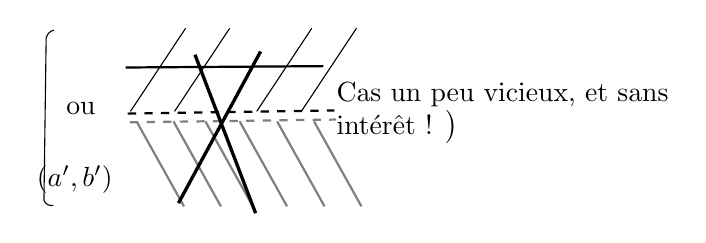
\begin{tikzpicture}[x=.70cm,y=.58cm]
\draw (-1.14,2.1) to[bend right=28](-1.28,1.93)--(-1.32,-1.63) to[bend right=38](-1.15,-1.74);
\node at (-.65,.38){ou};\node at (-.76,-1.18){$(a',b')$};
\draw[thick] (.16,1.28)--(3.75,1.31);\draw[thick,dashed] (.2,.27)--(3.95,.34);\draw[gray,thick,dashed] (.24,.08)--(3.98,.14);
\foreach \x in {.25,1.05,2.54,3.35}{\draw (\x,.32)--++(1,1.82);}
\foreach \x in {.36,1.03,1.61,2.23,2.91,3.58}{\draw[gray,thick] (\x,.1)--++(.86,-1.86);}
\draw[very thick] (1.42,1.56)--(2.52,-1.91) (1.12,-1.69)--(2.61,1.63);
\node[align=left] at (7,.28) {Cas un peu vicieux, et sans\\ intérêt ! $\big)$};
\end{tikzpicture}}

% @ L1–2, heading
\deleted{\unsure{4)|A)}} Cas $(a,b)$ \deleted{c'est le cas} de \uline{prolongation des rives}.

% @ L3–5
1) On choisit comme recollement le transport parallèle. On trouve un $\unsure{\mathscr X|X|\mathcal X}$ avec $\varphi:\mathscr X\to X$ qui est une immersion.

% @ L6–13
Dans $\mathscr X$, on a un graphe top. $K$, et les faces de $(\mathscr X,K)$ correspondent aux pos. stables. \deleted{\unsure{On a un}} On a un $L=\varphi^{-1}(X_1)$, qui matérialise la corr. entre faces et pos. stables -- en remplaçant chaque face $F$ par la face $F^{\sim}$ obtenue en la ``gonflant'' aux pts \deleted{qui} ``critiques'' de $\partial K$ i.e. les pts de $K\cap S(L)$.

% @ R1–7, main text
Partons d'une orientation $\omega=\underline\omega_F$ de $F=\Delta_D^*$, et d'un $\omega_D$ orientation de $D$, passant à l'orientation $\omega'$ de $\Delta_{D'}^*$ déduite par transport i.e. le vrillement, \deleted{\unsure{obte|obtient}} orientation $\omega_{D'}$ de $D'$, on constate encore que c'est l'\uline{opposé} de celle obtenue par transport parallèle !

% @ alongside R1–3 and R6–7
% slanted
\margin{\uline{NB} Ici, on \unsure{dilate|déduit} $\Delta_D^*$ en \unsure{prolongeant|prolg|prolonge} en $\unsure{D'|D|D_i}\cap\Delta_{D'}^*$}

\margin{L'ennui, c'est que les circuits sont \unsure{détestables|détables}. On n'obtient \ensuremath{=} pas les bons circuits supersinguliers !}

% @ R8–15
2) Recollement par l'iso $a\unsure{\simeq|\overset{\sim}{\longrightarrow}}b$ opposé au transport parallèle. Cette fois, c'est au niveau de la transition $\underline\omega_F$ \unsure{---,|---|\ensuremath{\to}} $\underline\omega_{F'}$, interprétée comme $\underline\omega_D$ --- $\underline\omega_{D'}$, qu'on obtient le transport parallèle. Contrairement à ce que je croyais, \inserted{encore hier} on trouve les bons circuits autour des positions supersingulières.
\scanpage{75}
% archive sheet number: 74
% @ L1–3
Mais les circuits plus généraux \deleted{\unsure{restent|restent-ils}} mystérieux pour moi -- je ne sais s'ils sont \unsure{bitables|bistables|bi-stables|valables} !

% @ L4–13
Les deux procédés correspondent à la $=$ structure polygonale sur l'\unsure{ens|un|ens.} des arcs de spécialisation \inserted{(= transition)} pour une pos. stable $D$ -- mais il y a une autre structure polygonale, due au fait que les \deleted{\unsure{uns des|arcs des}} arcs de spécialisation \uline{sur $D$} (au lieu de $\widetilde D$) sont naturellement disjoints, donc on peut prendre la structure polygonale correspondante, dont la réalisation top. est enc. $D$ lui-$=$. L'ennui, c'est que cette fois on a un polygône \deleted{\unsure{d'ordre algébrique}} \inserted{d'ordre $n$} non $2n$, \deleted{\unsure{dt|dont}} dont la signification géométrique des disques angulaires correspondants n'est pas claire. Mais peut-être est-ce une indication pour attacher \uline{simultanément} \uline{de deux façons} antipodiquement les disques $\Delta^*_{D},\Delta^*_{D'}$, de façon à obtenir un ruban de Möbius peut-être ?

% @ R1–6, with a lens-shaped drawing inside the sentence
L'idée maintenant, c'est de prendre la découpe de $X$ suivant la partie

\figure{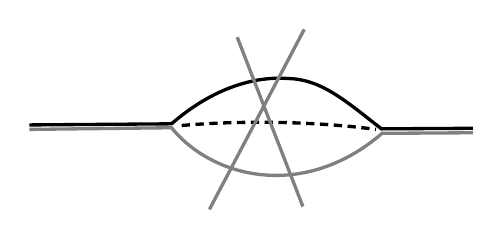
\begin{tikzpicture}[x=.86cm,y=.71cm]
\draw[very thick] (-3.5,0)--(-1.4,.02)..controls(-.85,.6)and(-.24,.88)..(.32,.83)..controls(.81,.82)and(1.17,.43)..(1.7,-.07)--(3.05,-.06);
\draw[gray,very thick] (-3.5,-.08)--(-1.4,-.05)..controls(-.8,-.95)and(.55,-1.36)..(1.71,-.15)--(3.05,-.14);
\draw[very thick,densely dashed] (-1.25,-.01)..controls(-.2,.1)and(.88,.04)..(1.62,-.08);
\draw[gray,very thick] (-.43,1.57)--(.54,-1.46) (.56,1.71)--(-.84,-1.51);
\end{tikzpicture}}

% @ R6–11 and notes within the lines
commune de $D$ et $D'$ (cf figure) ça donne donc un ruban de Möbius, \deleted{qu'on peut obtenir} \inserted{découpé par la ligne} pointillée en une bande rectangulaire. On prend le revêtement \deleted{\unsure{des}} \inserted{des orientations d'}ordre 2 du ruban de Möbius, \margin{(twisté par $\underline\omega(D)$ ?)} qui est formé de deux rectangles \unsure{vrillés|recollés} en 2 paires d'arêtes.

% @ R12–20
Sauf erreur, c'est l'identification \deleted{de} simultanée de \deleted{\unsure{$a'$|$a$}}\inserted{$a$} avec $b$, \deleted{\unsure{de|et}} \deleted{\unsure{$a$|$a'$}}\inserted{$a'$} avec $b'$, suivant le transport parallèle. Mais ce qu'on obtient, en faisant tous ces recollements pour l'ens. de tous les $\Delta_D^*$, est-elle bien la surface cellulaire obtenue par le graphe $\Gamma_{\unsure{\mathscr K|K|\Sigma}}$ et sa structure de polygonalisation et de transport ?, obtenue
\scanpage{76}
% archive sheet number: 75
% @ L1–11
par vrillement \uline{\unsure{de deux|des|deux|de}} polygones \uline{d'ordre $n$}, non $2n$ ? \deleted{\unsure{Cett|Cette|Celle}} La première ne serait-elle pas plutôt un revêtement d'ordre deux de la seconde, ramifiée en chacun des pts du centre -- en effet, on voit \deleted{apparemment} \inserted{que} les antipodismes des les $\Delta_D^*$ sont compatibles avec les identifications, -- par passage au quotient, cela va donner sûrement la carte cellulaire envisagée\ldots{}

% @ L11–20
On peut alors, \deleted{qui} après \deleted{\unsure{avoir enlevé|avoir admis}} interpréter la nouvelle carte comme associée à un graphe \inserted{(plongé cellulairement)} dont les sommets sont les pos. stables, qui pour deux pos. $D,D'$ adjacentes, on va maintenant envisager \uline{deux} flèches ou arêtes entre eux, savoir $a_D:D\mathbin{\text{---}}D'$ (de l'\unsure{about|arête} $a$ vers $b'$) et $a_{D'}:D'\mathbin{\text{---}}D$ (de l'\unsure{arête|autr} $b$ vers $a'$), munies chacune d'une orientation -- le balayage de $D$ vers $D'$, et de $D'$ vers $D$, qu'on désidentifie.

% @ R1–8
Maintnt, les arcs de transition (nouveau style) pour $D$ i.e. sur $\partial\Delta_D$, sont les arcs de spécialisation \uline{et leurs antipodiques}, organisés en polygône de la façon habituelle. On considère que par l'un ou par l'autre, on peut aller vers une position rel. \unsure{adjacentes|adjacente}.

% @ R9–15
La surface $\unsure{\mathscr X|X|\mathcal X}$ obtenue, immergée dans $X$ par une immersion, \deleted{\unsure{il|et}} l'image inverse \inserted{$L$} de $X_1$ \deleted{est} donne lieu à \deleted{une} l'interprétation habituelle \deleted{de} \unsure{la|fé.} \unsure{p.v.|pos.|p.r.} (stable) associée à une face de $(\mathscr X,K)$.

% @ R16–end, heading and list with brace
Description combinatoire

\[
\begin{aligned}
\text{1) graphe }\Gamma\quad\left\{\begin{aligned}
&\text{sommets : pos. stables }D\\
&\text{arêtes orientées : paires }(D,a),\ a\text{ un}\\
&\deleted{\text{ori.}}\qquad\text{arc de transition sur }D\\
&\qquad\text{(de spécialisation,}\\
&\qquad\text{ou antipodique}\\
&\qquad\text{d'un tel)}
\end{aligned}\right.
\end{aligned}
\]
